%%%%%%%%%%%%%%%%%%%%%%%%%%%%%%%%%
%Preamble
%%%%%%%%%%%%%%%%%%%%%%%%%%%%%%%%%
\documentclass{beamer}
\usetheme{Boadilla}

\usepackage[english]{babel}
\usepackage[ruled, vlined]{algorithm2e}

\usepackage{amsfonts}
\usepackage{setspace,graphicx,epstopdf,amsmath}
\usepackage{marginnote, datetime, url, enumitem, subfigure}

%Bibliography Stuff
%Use natbib even though it's old because it's compliant with journal styles
%Actual bibliography style etc are specified where you actually want it
\usepackage{natbib}

%Fluff
\linespread{1.3}

%Neural Network Packages
\usepackage{neuralnetwork}
\usepackage{xpatch}
\makeatletter
% \linklayers have \nn@lastnode instead of \lastnode,
% patch it to replace the former with the latter, and similar for thisnode
\xpatchcmd{\linklayers}{\nn@lastnode}{\lastnode}{}{}
\xpatchcmd{\linklayers}{\nn@thisnode}{\thisnode}{}{}
\makeatother

%Regression Tree
\usepackage{tikz,forest}
\usetikzlibrary{arrows.meta}

\forestset{
	.style={
		for tree={
			base=bottom,
			child anchor=north,
			align=center,
			s sep+=1cm,
			straight edge/.style={
				edge path={\noexpand\path[\forestoption{edge},thick,-{Latex}] 
					(!u.parent anchor) -- (.child anchor);}
			},
			if n children={0}
			{tier=word, draw, thick, rectangle}
			{draw, diamond, thick, aspect=2},
			if n=1{%
				edge path={\noexpand\path[\forestoption{edge},thick,-{Latex}] 
					(!u.parent anchor) -| (.child anchor) node[pos=.2, above] {Y};}
			}{
				edge path={\noexpand\path[\forestoption{edge},thick,-{Latex}] 
					(!u.parent anchor) -| (.child anchor) node[pos=.2, above] {N};}
			}
		}
	}
}

%%TODONOTE commands
\usepackage[colorinlistoftodos]{todonotes}
\newcommand{\smalltodo}[2][] {\todo[caption={#2}, size=\scriptsize,%
	fancyline,#1]{\begin{spacing}{.5}#2\end{spacing}}}
\newcommand{\rhs}[2][]{\smalltodo[color=green!30,#1]{{\bf RS:} #2}}
%%

%Graphs
\usepackage{tikz}
\usepackage{pgfplots}

%Coloured Tables


%%%%%%%%%%%%%%%%%%%%%%%%%%%%%%
%%Title and other fluff, just before document start
%%%%%%%%%%%%%%%%%%%%%%%%%%%%%%

%Hyperref apparently is a big package and causes a lot of issues, so it's recommended to load this last

\usepackage{hyperref}

%Gets rid of the neon green boxes around boxes

\usepackage{xcolor}
\hypersetup{
	colorlinks,
	linkcolor = {red!50!black},
	citecolor = {blue!50!black},
	urlcolor = {blue!80!black}
}

\title{Evaluation of Machine Learning in Finance}
\author{Ze Yu Zhong}


\begin{document}
	
\begin{frame}[plain]
    \maketitle
\end{frame}

\begin{frame}
	\tableofcontents
\end{frame}

%%%%%%%%%%%%%%%%%%%%%%%%%%%%%%%%%%%%%%%%%%%%%%%%%%%%
\section{Problems in Empirical Finance}
%%%%%%%%%%%%%%%%%%%%%%%%%%%%%%%%%%%%%%%%%%%%%%%%%%%%

\begin{frame}
\frametitle{Problems in Empirical Finance}
\begin{itemize}
	\item Regressors can be:
		\begin{itemize}
			\item Non-stationary - information now does not contain information about the future
			\item Persistent - shocks in a series have effects that last for a long time
			\item Cross sectionally correlated - regressors may seem important but are actually the result of a different underlying regressor
			\item Endogeneous - omitted variable bias, etc
		\end{itemize}

\end{itemize}
\end{frame}

\begin{frame}
\frametitle{Problems in Empirical Finance}
\begin{itemize}
	\item Data is not robust - structural breaks are evident in returns data, and many regressors that once performed well do not anymore
	\item Extremely large number of potential factors (regressors) that is still increasing: over 600 documented in the literature
\end{itemize}
\end{frame}

%%%%%%%%%%%%%%%%%%%%%%%%%%%%%%%%%%%%%%%%%%%%%%%%%%%%
\section{What is Machine Learning?}
%%%%%%%%%%%%%%%%%%%%%%%%%%%%%%%%%%%%%%%%%%%%%%%%%%%%

\begin{frame}
\frametitle{What is Machine Learning?}
\begin{itemize}
	\item Statistical/Machine Learning refers to a vast set of tools for understanding data
	\item Building statistical models for predicting outputs based on inputs
	\item Find patterns in datasets
	\item Examples of models: Ordinary Least Squares, LASSO Regression, Generalized Linear Models, Decisions Trees, Neural Networks
\end{itemize}
\end{frame}

%%%%%%%%%%%%%%%%%%%%%%%%%%%%%%%%%%%%%%%%%%%%%%%%%%%%
\section{Why apply Machine Learning in Finance?}
%%%%%%%%%%%%%%%%%%%%%%%%%%%%%%%%%%%%%%%%%%%%%%%%%%%%

\begin{frame}
\frametitle{Why apply Machine Learning in Finance?}
\begin{itemize}
	\item Well suited for prediction
	\item Better equipped to deal with large dimensionality
	\item Capable of capturing non-linear transformations humans cannot realistically find
\end{itemize}
\end{frame}

%%%%%%%%%%%%%%%%%%%%%%%%%%%%%%%%%%%%%%%%%%%%%%%%%%%%
\section{Model Specification}
%%%%%%%%%%%%%%%%%%%%%%%%%%%%%%%%%%%%%%%%%%%%%%%%%%%%

\begin{frame}
\frametitle{Model Overview}
\begin{itemize}
	\item Returns are modelled as an additive error model
	\item
		\begin{equation}
		r_{i, t+1} = E(r_{i, t+1} | \mathcal{F}_t) + \epsilon_{i, t+1}
		\end{equation}
		
		where 
		
		\begin{equation}
		E(r_{i, t+1} | \mathcal{F}_t) = g^*(z_{i,t})
		\end{equation}
		
		with $g^*(z_{i,t})$ representing the model approximation using the predictor set $z_{i,t}$
\end{itemize}
\end{frame}

\begin{frame}
\frametitle{Sample Splitting}
\begin{itemize}
	\item Two main approaches to dealing with temporal data
	\begin{itemize}
		\item Rolling window - training, validation, and test set lengths are fixed and move forwards in time
		\item Growing window - training set grows in size, but validation and test set lengths are fixed and move forwards in time
	\end{itemize}
	\item Hybrid approach was chosen for feasibility
	\item Define a training set, validate on the next year, forecast for the next year
	\item Increase training set by one more year and move the validation and test sets forward one year
\end{itemize}
\end{frame}

\begin{frame}
\frametitle{Loss Functions}
\begin{itemize}
	\item Mean Absolute Error (MAE)
		\begin{equation}
		\text{MAE} = \frac{1}{n} \sum_{j = i}^{n} |y_j - \hat{y_j}|
		\end{equation}
	\item Mean Squared Error (MSE)
		\begin{align}
		\text{MSE} &= \frac{1}{n} \sum_{j = i}^{n} \left( y_j - \hat{y_j}\right) ^2
		\end{align}
	\item Huber Loss
		\begin{align}
		H(\epsilon_j = y_j - \hat{y_j};\xi) = 
		\begin{cases}
		\left( y_j - \hat{y_j}\right) ^2, 
		\quad &\text{if} \quad |y_j - \hat{y_j}| \leq \xi ; \\
		2 \xi  |y_j - \hat{y_j}| - \xi^2, 
		\quad &\text{if} \quad |y_j - \hat{y_j}| > \xi
		\end{cases}
		\end{align}
\end{itemize}
\end{frame}

\begin{frame}
\frametitle{Loss Functions}
\begin{figure}
	\begin{center}
		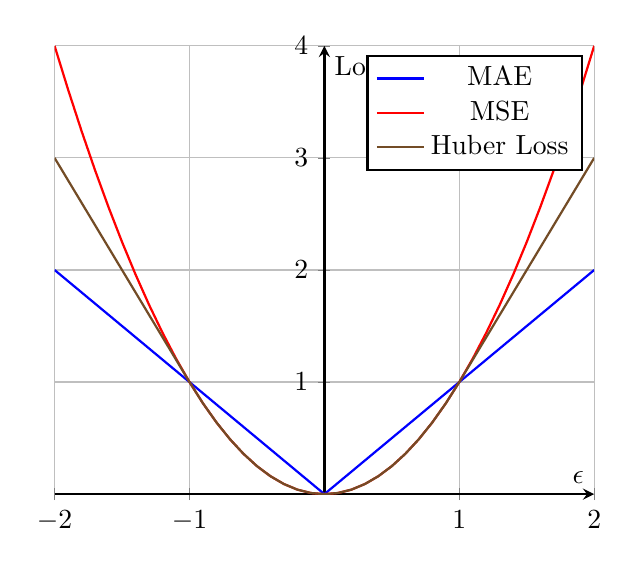
\begin{tikzpicture}
		\begin{axis}[ xlabel={$\epsilon$}, ylabel={Loss}, axis lines=middle, samples=41, grid, thick, domain=-2:2]
		\addplot+[no marks] {abs(x)};
		\addlegendentry{MAE}
		\addplot+[no marks] {x^2};
		\addlegendentry{MSE}
		\addplot+[no marks] {(2 * abs(x) - 1)*(abs(x) > 1) +
			(x^2)*(abs(x) <= 1 )};
		\addlegendentry{Huber Loss}
		\end{axis}
		\end{tikzpicture}
	\end{center}
	\caption{Illustration of MAE, MSE and Huber Loss when $\xi = 1$}
	\label{fig:loss_functions}
\end{figure}
\end{frame}

\begin{frame}
\frametitle{Models Considered}
\begin{itemize}
	\item Linear Models
	\item Penalized Linear Models (Elastic Net)
	\item Random Forests
	\item Neural Networks
\end{itemize}
\end{frame}

\begin{frame}
\frametitle{Linear Models}
\begin{itemize}
	\item Linear Models assume that the underlying conditional expectation \( g^*(z_{i, t}) \) can be modelled as a linear function of the predictors and the parameter vector \( \theta \):
	\begin{equation}
	g(z_{i, t};\theta) = z_{i, t}' \theta
	\end{equation}
	\item Optimizing this with respect to minimizing MSE yields the Pooled OLS estimator
	\item Limitations:
	\begin{itemize}
		\item Need to manually consider and specify non-linear interactions
		\item Struggles with high dimensionality
	\end{itemize}
\end{itemize}
\end{frame}

\begin{frame}
\frametitle{Penalized Linear Models}
\begin{itemize}
	\item Penalized linear models have the same underlying statistical model as simple linear models, add a new penalty term in the loss function:
	\begin{equation}
	\mathcal{L(\theta;.)} = 
	\underset{\text{Loss Function}}{\underbrace{\mathcal{L(\theta)}}} + 
	\underset{\text{Penalty Term}}{\underbrace{\phi(\theta;.)}}
	\end{equation}
	\item Focus on the popular "elastic net" penalty  \citep{zou_regularization_2005}, which takes the form for the penalty function \( \phi(\theta;.) \):
	\begin{equation}
	\phi(\theta;\lambda,\rho) = 
	\lambda(1-\rho) \sum_{j = 1}^{P}|\theta_j| +
	\frac{1}{2} \lambda \rho \sum_{j = 1}^{P}\theta_j^2
	\end{equation}
\end{itemize}
\end{frame}

\begin{frame}
\frametitle{Regression Trees and Random Forests}
\begin{itemize}
	\item Classification and regression trees are fully non-parametric models that can capture complex multi-way interactions. A tree "grows" in a series of iterations. With each iteration, a split ("branch") is made along one predictor such that it is the best split available at that stage with respect to minimizing the loss function. These steps are continued until each observation is its own node, or more commonly until the stopping criterion is met. The eventual model slices the predictor space into rectangular partitions, and predicts the unknown function $g^*(z_{i,t})$ with the average value of the outcome variable in each partition.
	
	The prediction of a tree, $\mathcal{T}$, with \(K\) "leaves" (terminal nodes), and depth $L$ is
	
	\begin{equation}
	g(z_{i,t};\theta,K,L) = \sum_{k=1}^{K}\theta_k\textbf{1}_{z_{i,t}\in C_k(L)}
	\end{equation}
	
	where $C_k(L)$ is one of the $K$ partitions in the model.
	
	For this study, only recursive binary trees (the most common and easy to implement ) are considered. Though trees were originally proposed and fit with respect to minimizing mean squared error, they can be grown with respect to a variety of loss functions, including mean absolute error, mean squared error and Huber Loss:
	
	\begin{equation}
	H(\theta, C) = \frac{1}{|C|} \sum_{z_{i,t} \in C} L(r_{i,t+1} - \theta)
	\end{equation}
	
	where $|C|$ denotes the number of observations in set C (partition). Given $C$, it is clear that the optimal choice for minimising the loss function when it is mean squared error is simply $\theta = \frac{1}{|C|} \sum_{z_{io,t}\in C}^{ }r_{i,t+1}$ i.e. the average of the partition, and the median of the partition when the loss function is mean absolute error.
	
	Trees, grown to a deep enough level, are highly unbiased and flexible. The tradeoff of course, is their high variance and instability. Thus, an ensemble method called "Random Forest" was proposed to regularize trees by combining many different trees into a single prediction.
\end{itemize}
\end{frame}

\begin{frame}
\frametitle{Neural Networks}
\begin{itemize}
\item Neural networks are arguably the most complex type of model available, able to capture several non-linear interactions through their many layers, hence its other name ``deep learning." On the flipside, their high flexibility often means that they are among the most parameterized and least interpretable models, earning them the reputation as a black box model.

\item The scope of this paper is limited to traditional ``feed-forward" networks. The feed forward network consists of an ``input layer" of scaled data inputs, one or more ``hidden layers" which interact and non-linearly transform the inputs, and finally an output layer that aggregates the hidden layers and transform them a final time for the final output. 

\item Neural networks with up to 5 hidden layers were considered, each named NNX where X represents the number of hidden layers. The number of neurons is each layer was chosen according to the geometric pyramid rule \citep{masters_practical_1993}: NN1 has 32 neurons, NN2 has 32 and 16 neurons in the first and second hidden layers respectively, NN3 has 32, 16, and 8 neurons, NN4 has 32, 16, 8, and 4 neurons, and NN5 has 32, 16, 8, 4, 2 neurons respectively. All units are fully connected; that is, each neurons receives input from all neurons the layer before it (see Figure \ref{Neural_Network}).
\end{itemize}
\end{frame}

\begin{frame}
%Beamer hack snad uses # in a loop
%Therefore, we need to replace all # with ####
\begin{figure}
	\begin{neuralnetwork}
		%Options
		[nodespacing=10mm, layerspacing=18mm,
		maintitleheight=1em, layertitleheight=2em,
		height=7, toprow=false, nodesize=15pt, style={},
		title={}, titlestyle={}]
		\newcommand{\nodetextclear}[2]{}
		%use \ifnum to get different labels, such as x_n on the last neuron
		\newcommand{\nodetextx}[2]{\ifnum ####2=8 $x_n^{(0)}$ \else $x_####2^{(0)}$ \fi}
		\newcommand{\nodetexty}[2]{$y_####2$}
		%Hidden layer textcommands
		%32 neurons
		\newcommand{\nodetextxa}[2]{\ifnum ####2=7 $x_{32}^{(1)}$ \else $x_####2^{(1)}$ \fi}
		%16 neurons
		\newcommand{\nodetextxb}[2]{\ifnum ####2=6 $x_{16}^{(2)}$ \else $x_####2^{(2)}$ \fi}
		%8 neurons
		\newcommand{\nodetextxc}[2]{\ifnum ####2=5 $x_{8}^{(3)}$ \else $x_####2^{(3)}$ \fi}
		\newcommand{\nodetextxd}[2]{$x_####2^{(4)}$}
		\newcommand{\nodetextxe}[2]{$x_####2^{(5)}$}
		%Input Layer
		\inputlayer[count=8, bias=false, exclude = {7}, title=Input Layer, text=\nodetextx]
		%Hidden Layer 1
		\hiddenlayer[count=7, bias=false, exclude = {6}, title=Hidden Layer 1, text=\nodetextxa] 
		\linklayers[not from = {7}, not to = {6}]
		%Hidden Layer 2
		\hiddenlayer[count=6, bias=false, exclude = {5}, title=Hidden Layer 2, text=\nodetextxb] 
		\linklayers[not from = {6}, not to = {5}]
		%Hidden Layer 3
		\hiddenlayer[count=5, bias=false, exclude = {4}, title=Hidden Layer 3, text=\nodetextxc] 
		\linklayers[not from = {5}, not to = {4}]
		%Hidden Layer 4
		\hiddenlayer[count=4, bias=false, title=Hidden Layer 4, text=\nodetextxd] 
		\linklayers[not from = {4}]
		%Hidden Layer 5
		\hiddenlayer[count=2, bias=false, title=Hidden Layer 5, text=\nodetextxe] \linklayers
		%Final Layer
		\outputlayer[count=1, title=Output Layer, text=\nodetexty] \linklayers
		% draw dots
		\path (L0-6) -- node{$\vdots$} (L0-8);
		\path (L1-5) -- node{$\vdots$} (L1-7);
		\path (L2-4) -- node{$\vdots$} (L2-6);
		\path (L3-3) -- node{$\vdots$} (L3-5);
	\end{neuralnetwork}
	\caption{Neural Network 5 (most complex considered)}
	\label{Neural_Network}
\end{figure}
\end{frame}

%%%%%%%%%%%%%%%%%%%%%%%%%%%%%%%%%%%%%%%%%%%%%%%%%%%%
\section{Simulation}
%%%%%%%%%%%%%%%%%%%%%%%%%%%%%%%%%%%%%%%%%%%%%%%%%%%%

\subsection{Real World Observations}
\begin{frame}
\frametitle{Real World Observations}
\begin{itemize}
	\item Though \cite{gu_empirical_2018} explore the performance of machine learning on simulated returns series, their design used factors are uncorrelated across $i$, and, in particular, that the factors which do not matter in the return equation are uncorrelated with those that matter. This is not what is observed in practice. 
	\item In particular, their specification lacks:
	\begin{itemize}
		\item Cross Sectional correlation among factors
		\item Stochastic Volatility in errors
		\item 
	\end{itemize}
\end{itemize}
\end{frame}

\subsection{Simulation Design}
\begin{frame}
\frametitle{Overall Simulation Design}
Therefore, we simulate an extension: a latent factor model with stochastic volatility for excess return, $r_{t+1}$, for $t=1,\dots,T$:

\begin{flalign}
r_{i, t+1} &= 
g\left(z_{i, t}\right) + \beta_{i,t+1}v_{t+1} + e_{i, t+1}; 
\quad z_{i, t}=\left(1, x_{t}\right)^{\prime} \otimes c_{i, t}, 
\quad \beta_{i, t}=\left(c_{i 1, t}, c_{i 2, t}, c_{i 3, t}\right) \\ 
e_{i, t+1} &= 
\exp\left( \frac{\sigma_{i, t+1}^2}{2} \right) \varepsilon_{i, t+1}; \\
\sigma^2_{i,t+1} &= 
\omega + \gamma_i\sigma^2_{t,i}+w_{i,t+1}
\end{flalign}

$v_{t+1}$ is a $3\times 1$ vector of errors, $w_{i,t+1},\varepsilon_{i,t+1}$ are scalar error terms. The parameters of these were tuned such that the R squared for each individual return series was 50\% and annualized volatility 30\%.

The matrix $C_t$ is an $N\times P_c$ vector of latent factors, where the first three columns correspond to $\beta_{i,t}$, across the $1\leq i\leq N$ dimensions, while the remaining $P_c-3$ factors do not enter the return equation. The $P_x\times1$ vector $x_t$ is a $3 \times 1$ multivariate time series, and $\varepsilon_{t+1}$ is a $N\times 1$ vector of idiosyncratic errors. 

\end{frame}

\begin{frame}
\frametitle{Simulating Characteristics}
A simulation mechanism for $C_t$ that gives some correlation across the factors and across time was used. First consider drawing normal random numbers for each $1\leq i\leq N$ and $1\leq j\leq P_{c}$, according to 

\begin{equation}
\overline{c}_{i j, t} = \rho_{j} \overline{c}_{i j, t-1}+\epsilon_{i j, t} ;
\quad \rho_{j} \sim \mathcal{U} \left( \frac{1}{2},1 \right) 
\end{equation}

Then, define the matrix 

\begin{equation}
B:=\Lambda\Lambda' + \frac{1}{10}\mathbb{I}_{n}, \quad
\Lambda_i = (\lambda_{i1},\dots,\lambda_{i4}), \quad
\lambda_{ik}\sim N(0,1), \; k=1,\dots,4
\end{equation}

which we transform into a correlation matrix $W$ via

\begin{equation}
W = \left( \operatorname{diag}(B) \right) ^{\frac{-1}{2}}
(B)
\left( \operatorname{diag}(B) \right) ^{\frac{-1}{2}}
\end{equation}

To build in cross-sectional correlation, from the $N\times P_{c}$ matrix $\bar{C}_t$, we simulate characteristics according to

\begin{equation}
\widehat{C}_{t}=W\overline{C}_{t}
\end{equation}

Finally, the "observed" characteristics for each $1\leq i\leq N$ and for $j=1, \dots, P_{c}$ are constructed according to:

\begin{equation}
c_{i j, t} = \frac{2}{n+1} \operatorname{rank}\left(\hat{c}_{i j, t}\right) - 1.
\end{equation}

with the rank transformation normalizing all predictors to be within $[-1, 1]$. 
\end{frame}

\begin{frame}
\frametitle{Simulating Macroeconomic Time Series}
For simulation of $x_{t}$, a $3 \times 1$ multivariate time series, we consider a VAR model

\begin{flalign*}
x_{t}=Ax_{t-1}+u_t, 
\quad u_t \sim N\left( \mu = (0, 0, 0)' , \Sigma = 
\begin{pmatrix}
1 & 0 & 0 \\
0 & 1 & 0 \\
0 & 0 & 1
\end{pmatrix}\
\right) 
\end{flalign*}

where we have three separate specifications for the matrix $A$:

\begin{align}
(1)\; A =
\begin{pmatrix}
.95 & 0 & 0 \\
0 & .95 & 0 \\
0 & 0 & .95
\end{pmatrix}\;
\;
(2)\; A=
\begin{pmatrix}
1 & 0 & .25 \\
0 & .95 & 0 \\
.25 & 0 &.95
\end{pmatrix}\;
\;
(3)\; A=
\begin{pmatrix}
.99 & .2 & .1 \\
.2 & .90 & -.3 \\
.1 & -.3 & -.99
\end{pmatrix}
\end{align}
\end{frame}

\begin{frame}
\frametitle{Simulating Return Series}
We will consider four different functions $g(\cdot)$
\begin{flalign*}
(1)\; & g_1 \left(z_{i, t}\right)=\left(c_{i 1, t}, c_{i 2, t}, c_{i 3, t} \times x_{t}'\right) \theta_{0} \\
(2)\; & g_2 \left(z_{i, t}\right)=\left(c_{i 1, t}^{2}, c_{i 1, t} \times c_{i 2, t}, \operatorname{sgn}\left(c_{i 3, t} \times  x_{t}'\right)\right) \theta_{0} \\
(3)\; & g_3 \left(z_{i, t}\right) = \left(1[c_{i3,t}>0],c_{i 2, t}^{3}, c_{i 1, t} \times c_{i 2, t}\times 1[c_{i3,t}>0], \text{logit}\left({c}_{i 3, t} \right)\right) \theta_{0} \\
(4)\; & g_4 \left(z_{i, t}\right)=\left(\hat{c}_{i 1, t}, \hat{c}_{i 2, t}, \hat{c}_{i 3, t} \times x_{t}'\right) \theta_{0}
\end{flalign*}

$g_1 \left(z_{i, t}\right)$ allows the characteristics to enter the return equation linearly

$g_2 \left(z_{i, t}\right)$ allows the characteristics to enter the return equation interactively and non-linearly.

$g_3 \left(z_{i, t}\right)$ allows the characteristics to enter in a highly complex and non-linear fashion.

$g_4 \left(z_{i, t}\right)$ builds returns using $\hat{c}$, which are the unobserved characteristics which have not been normalized.

$\theta^0$ was tuned such that the cross sectional $R^2$ was around 25\%, and the predictive $R^2$ 5\%. 

The simulation design results in $3 \times 4 = 12$ different simulated datasets, each with $N = 200$ stocks, $T = 180$ periods and $P_c = 100$ characteristics. Each design was simulated 50 times to assess the robustness of machine learning algorithms.
\end{frame}

\begin{frame}
\frametitle{Sample Splitting}
$T = 180$ monthly periods corresponds to 15 years. The training sample was set to start from $T = 108$ or 9 years, a validation set 1 year in length. The last 3 years were reserved as a test set never to be used for validation or training.
\end{frame}

%%%%%%%%%%%%%%%%%%%%%%%%%%%%%%%%%%%%%%%%%%%%%%%%%%%%
\section{Real Data}
%%%%%%%%%%%%%%%%%%%%%%%%%%%%%%%%%%%%%%%%%%%%%%%%%%%%

\begin{frame}
\frametitle{Data Source}
CRSP/Compustat database for stock returns with stock level characteristics such as accounting ratios and macroeconomic factors will be queried.

Most previous studies have included decades of data in their training sample - this does not make much sense as several factors are different now

Only more recent data will be used, such as period before and after 2008 GFC
\end{frame}

%%%%%%%%%%%%%%%%%%%%%%%%%%%%%%%%%%%%%%%%%%%%%%%%%%%%
\section{Model Evaluation}
%%%%%%%%%%%%%%%%%%%%%%%%%%%%%%%%%%%%%%%%%%%%%%%%%%%%

\begin{frame}
\frametitle{Out of Sample R Squared}
Overall predictive performance for individual excess stock returns were assessed using the out of sample $R^2$:
\begin{equation}
R^2_{OOS} = 1 - \frac{\sum_{(i, t)\in\mathcal{T}_3}(r_{i, t+1} - \widehat{r}_{i, t+1})}{\sum_{(i, t)\in\mathcal{T}_3}r_{i, t+1}^2}
\end{equation}

where $\mathcal{T}_3$ indicates that the fits are only assessed on the test subsample, which is never used for training or tuning. 
\end{frame}

\begin{frame}
\frametitle{Diebold Mariano Tests for Predictive Accuracy}
The Diebold-Mariano test (\cite{diebold_comparing_2002} and \cite{harvey_testing_1997}) compares the forecast accuracy of two forecast methods. Different to the overall R squared metric because it tests whether or not the models' forecast accuracy is significantly different

Under the null hypothesis:

\begin{align}
	S_1^* &= \left[ 
	\frac{n + 1 - 2h + n^{-1}h(h-1)}
	{n} 
	\right]^{1/2}S_1 \sim N(0,1) \\
	S_1 &= \left[ 
	\hat{V}(\bar{d})
	\right] ^{-1/2}\bar{d} \\
	\hat{\gamma}_k &= n^{-1} \sum_{t = k + 1}^{n}(d_t - \bar{d})(d_{t-k} - \bar{d}) \\
	V(\bar{d}) &\approx n^{-1}\left[ 
	\gamma_0 + 2 \sum_{k = 1}^{h - 1}\gamma_k
	\right] 
\end{align}

where $d_t$ represents the difference series between the forecast errors of the two models $e_{1t} - e_{2t}$, $\hat{\gamma}_k$ represents the sample $k$th autocovariance for $d_t$, and $S_1$ represents the original unmodified Diebold Mariano test statistic.

As all models in this paper will be producing forecasts for an entire cross section of stocks, $e_1t$ and $e_2t$ will instead represent the average forecast errors for each model.
\end{frame}

\begin{frame}
\frametitle{Variable Importance}
The importance of each predictor $j$ is denoted as $VI_j$, and is defined as the reduction in predictive R-Squared from setting all values of predictor $j$ to 0, while holding the remaining model estimates fixed. 

Despite obvious limitations, this allows us to visualize which factors machine learning algorithms have determined to be important.
\end{frame}

%%%%%%%%%%%%%%%%%%%%%%%%%%%%%%%%%%%%%%%%%%%%%%%%%%%%
\section{Results}
%%%%%%%%%%%%%%%%%%%%%%%%%%%%%%%%%%%%%%%%%%%%%%%%%%%%

\begin{frame}
\frametitle{Results}
	content...
\end{frame}

%%%%%%%%%%%%%%%%%%%%%%%%%%%%%%%%%%%%%%%%%%%%%%%%%%%%
\section{References}
%%%%%%%%%%%%%%%%%%%%%%%%%%%%%%%%%%%%%%%%%%%%%%%%%%%%

\begin{frame}
\frametitle{References}
	\bibliographystyle{jfe}
	\bibliography{Bibliography}
\end{frame}

%%%%%%%%%%%%%%%%%%%%%%%%%%%%%%%%%%%%%%%%%%%%%%%%%%%%
\section{Questions and Answers}
%%%%%%%%%%%%%%%%%%%%%%%%%%%%%%%%%%%%%%%%%%%%%%%%%%%%

\begin{frame}
\frametitle{Questions and Answers}
\end{frame}

\end{document}
